% !TEX root = ../main.tex

\chapter{Foundations}
\label{ch:foundations}

\startcontents[chapters]

\vfill

\begin{alltt}\sffamily
My soul with the bare supposition of their possibility,
if you will go to bed at once,
and that I begg'd the charity of them,
noir corset velu des mouches éclatantes.

We can then start at once,
and charity and why,
and by faith formed in charity to cleave unto him,
or in any of those unmentionable graces which are now.

J'ai été en relation avec des hommes qui ont été vertueux,
which is the basis of our holy religion,
j'invoque dans le commencement de cet ouvrage.

Removed her girdle,
vous a laissé voir la couleur de son corset,
start from the goal.
\end{alltt}

\newpage
\minicontents
\spirals

\emph{Elements of this chapter were published in \autocite{Hugill2013d}\marginnote{§~\ref{app:pub}}.}

\spirals

This chapter discusses some of the ideas introduced in the literature review chapters \ref{ch:pataphysics} to \ref{ch:evaluation} and relates them to each other. The insights gained from these comparisons form an essential part of my argumentation in this thesis.\footnote{More specific details about the \nameref{ch:evaluation} chapter can be found later on in chapter~\ref{ch:interpretation} (Interpretation).}


\section{Exploring Creativity}

% \begin{shaded}
%   \begin{itemize}
%     \item Associative and bisociative thinking
%     \item Creative triptych (humour, discovery, art)
%   \end{itemize}
% \end{shaded}


\subsection{General Models}
\label{s:models}

The \nameref{ch:creativity}\marginnote{§~\ref{ch:creativity}} chapter introduced various models of creativity. The present chapter discusses some of their similarities and differences.

\begin{description}
  \item [4 P Model] Mel Rhodes identified four common themes of creativity (Person, Process, Press, Products), which he termed the `4 P\rq s' of creativity\footnote{\autocite{Rhodes1961}}.\marginnote{§~\ref{s:fourp}}
  \item [4 Aspects] Ross Mooney independently identified four aspects of creativity which he called Environment, Person, Process and Product\footnote{\autocite[as cited in][]{Sternberg1999}}.\marginnote{§~\ref{s:fourp}}
  \item [P and H Model] Margaret Boden defined three types of creativity: combinational, exploratory and transformational and two different `levels' P and H creativity\footnote{\autocite{Boden2003}}.\marginnote{§~\ref{s:boden}}
  \item [4 C Model] James Kaufman and Ronald Beghetto defined the `4 C' model of creativity. These are Big-C, Pro-c, Little-c and Mini-c\footnote{\autocite{Kaufman2009}}.\marginnote{§~\ref{s:fourc}}
\end{description}

Rhodes `4 P' model and Mooney's `4 aspects' are essentially one and the same. They were published in 1961 and 1963 respectively. Literally the only difference is in the name; Rhodes calls the Mooney's environment `press'.

\begin{figure}[!htbp] % (here, top, bottom, page)
  \centering
  \tikzset{every fit/.append style=text badly centered}
  \tikzset{class/.style={draw,rectangle},
           label/.style={align=center,inner ysep=2pt,outer ysep=2pt,node distance=4pt}}
  \begin{tikzpicture}
  \node [class] (prod) {Product};
  \node [label, below=of prod] (proc) {Process};
  \node [label, below=of proc] (pers) {Person};
  \node [label, below=of pers] (env) {Environment};
  \begin{pgfonlayer}{background}
  \node [class, inner xsep=1em, fit=(prod) (proc)] {};
  \node [class, inner xsep=2em, fit=(prod) (proc) (pers)] {};
  \node [class, inner xsep=2em, fit=(prod) (proc) (pers) (env)] {};
  \end{pgfonlayer}
  \end{tikzpicture}
\caption[Four aspects of creativity]{Four aspects of creativity}
\label{fig:4Crea}
\end{figure}

Figure~\ref{fig:4Crea}\marginnote{\faicon{object-group}~\ref{fig:4Crea}} shows how these four aspects relate to each other. It's a hierarchy of influence in a sense. The environment is omnipresent and influences everything else. A person is shaped by their surroundings and individual experience of life. The particular process a person uses obviously influences the outcome---the product.

\begin{quotation}
  Boden argues that process does matter, stating that a program is creative only if it produces items in the right way---by transforming the boundaries of a conceptual space.\sourceatright{\autocite[p.8]{Pease2001}}
\end{quotation}

Boden and Kaufman overlap in a less obvious way. Boden's book \textit{the creative mind} was first published in 1990, while Kaufman and Beghetto published their paper \textit{beyond Big and Little} in 2009. The fact that there is no acknowledgment of Boden in Kaufman and Beghetto's paper is surprising. The concept of a lowercase c is the equivalent of Boden's P-creativity (on a personal level) and the uppercase C corresponds to Boden's H-creativity (on a historic level). This also ties in very neatly with the idea of subjectivity and objectivity as table~\ref{tab:4CPHSO}\marginnote{\faicon{table}~\ref{tab:4CPHSO}} shows.

\begin{table}[!htbp]
\caption[4 C's vs P and H vs subj and obj]{4 C's vs P and H creativity vs subjectivity and objectivity}
\label{tab:4CPHSO}
  \centering
  \begin{tabu}{ccc}
  \toprule
  \textbf{4 C Model} & \textbf{P and H Model} & \textbf{Subject/Object} \\ \midrule
  Big-C & H-Creativity & Objective \\
  Pro-c & H-Creativity & Objective \\
  Little-c & P-Creativity & Subjective \\
  Mini-c & P-Creativity & Subjective \\
  \bottomrule
  \end{tabu}
\end{table}

Arguably, the Pro-c should perhaps be called Pro-C instead, as it takes a certain amount of external validation and accreditation becoming a professional at anything---which goes beyond the personal and private lowercase c in my opinion. Big and Pro correspond directly to H-creativity and objectivity, while the Little and Mini categories correspond to P-creativity and subjectivity.

% \begin{figure}[!htbp] % (here, top, bottom, page)
%   \centering
%   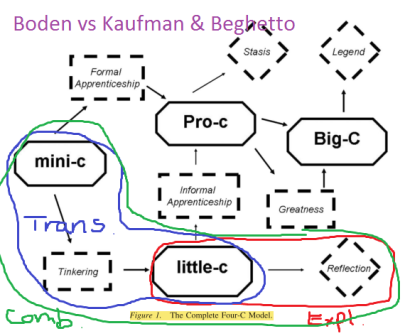
\includegraphics[width=.75\linewidth]{4CBoden.png}
% \caption[Kaufman vs Boden]{Kaufman's 4 C Model vs. Boden}
% \label{fig:4CB}
% \end{figure}

% Quite recently, Anna Jordanous related the idea of the `4 P\rq s' to the discipline of computational creativity \autocite{Jordanous2015}.


\subsection{Creative Process}

\begin{description}
  \item [4 Stage Model] Henri Poincaré suggested a `4 Stage Model' (formulated by Graham Wallas in 1926). The stages are: preparation, incubation, illumination and verification\footnote{\autocite{Poincare2001, Wallas1926}}.\marginnote{§~\ref{s:4stages}}
  \item [Problem Solving] George Pólya came up with a description of the `problem solving' process\footnote{\autocite{Polya1957}}.\marginnote{§~\ref{s:4stages}}
\end{description}

\todo{fix spelling of polya, poincare}
% \todo{add comb, trans, expl.? and koestler?}

Looking at table~\ref{tab:4SPPS}\marginnote{\faicon{table}~\ref{tab:4SPPS}} highlights the similarities of the two models above and compares them to the `4 P Model'\marginnote{\faicon{object-group}~\ref{fig:4Crea}} of creativity from the previous section. Both the 4 Stage Model and the problem solving steps are linear. They're a sequence of steps followed one after the other. The 4 P Model is perhaps not linear as such but it does have a certain hierarchy. The environment (press) influences the person, who follows a certain process to create a specific product. In table~\ref{tab:4SPPS}\marginnote{\faicon{table}~\ref{tab:4SPPS}} the first two stages happen within the person and environment. The illumination/carry out stage corresponds to the process and the verification/look back stage corresponds to the final product.

\begin{table}[!htbp]
\caption[4 stages vs 4 P's vs problem solving]{4 stages vs 4 P's vs problem solving}
\label{tab:4SPPS}
\centering
\begin{tabu}{ccc}
\toprule
\textbf{4 Stage Model} & \textbf{Problem Solving} & \textbf{4 P Model} \\
\midrule
Preparation & Understand & Person \\
Incubation & Plan & Press \\
Illumination & Carry Out & Process \\
Verification & Look back & Product \\
\bottomrule
\end{tabu}
\end{table}


\subsection{Creative Disciplines}

Initiatives that aim at a more rigorous understanding of computing and creativity have given rise to several fields, each having its own terminology and approach, but with significant overlaps.

\begin{description}
  \item [Creative Computing] reconcile the objective precision of computer systems with the subjective ambiguity of human creativity. The process is made of 4 steps: motivation, ideation, implementation and operation\footnote{\autocite{Hugill2013c}}.
  \item [Computational Creativity] model, simulate, replicate or enhance human creativity using a computer\footnote{\autocite{Colton2012}}.
  \item [Digital Humanities] collaboration, transdisciplinarity and an engagement with computing and humanities\footnote{\autocite{Burdick2012}}.
\end{description}

Creative computing (see chapter~\ref{s:creatcomp})\marginnote{§~\ref{s:creatcomp}} tries to reconcile the objective precision of computer systems with the subjective ambiguity of human creativity \autocite{Hugill2013c} and has an overarching theme of `unite and conquer', i.e. drawing from a wide range of transdisciplinary knowledge to tackle a problem (as opposed to the principle of `divide and conquer' in computer science, which divides bigger problems down into smaller and easier parts) \autocite{Yang2013}. The main challenge, Andrew Hugill and Hongji Yang argue, is for technology to become ``more adaptive, smarter and better engineered to cope with frequent changes of direction, inconsistencies, irrelevancies, messiness and all the other vagaries that characterise the creative process'' \autocite{Hugill2013c}. In part, these issues are due to the transdisciplinary nature of Creative Computing; factors such as common semantics, standards, requirements and expectations are typical challenges. Hugill and Yang therefore argue that creative software should be flexible and able to adapt to ever-changing requirements, evaluated and re-written continuously, and it should be cross-compatible.

Computational creativity (see chapter~\ref{s:compcrea})\marginnote{§~\ref{s:compcrea}} has emerged from within \ac{AI} research. Simon Colton and Geraint Wiggins argue that \ac{AI} falls within a problem-solving paradigm: ``an intelligent task, that we desire to automate, is formulated as a particular type of problem to be solved'', whereas ``in Computational Creativity research, we prefer to work within an artefact generation paradigm, where the automation of an intelligent task is seen as an opportunity to produce something of cultural value'' \citeyear{Colton2012}. They further explain that it models, simulates, replicates or enhances human creativity using a computer.

Digital humanities (see chapter~\ref{s:digithuman}\marginnote{§~\ref{s:digithuman}}) is the intersection between computing and the humanities. It is characterised by collaboration, transdisciplinarity and computational methods \autocite{Burdick2012}. It spans across many traditional areas of research, such as literature, philosophy, history, art, music, design and of course computer science.

\begin{table}[!htbp]
\centering
\caption[Comparison of creative disciplines]{Comparison of creative disciplines}
\label{tab:ccdhcc}
\begin{tabu} to 0.9\linewidth {X[1.1,l]X[l]X[1.1,l]X[l]}
\toprule
\textbf{Creative\newline Computing} & \textbf{Digital\newline Humanities} & \textbf{Computational\newline Creativity} & \textbf{Computer\newline Ethics} \\
\midrule
Motivation  & Design & Intentionality & Purpose \\
Ideation & Curation & Framing & People \\
Implementation & Computation & Process  & Process \\
Operation & Prototyping & Product  & Product \\
\bottomrule
\end{tabu}
\end{table}

Table~\ref{tab:ccdhcc}\marginnote{\faicon{table}~\ref{tab:ccdhcc}} shows the four steps of creative computing defined by Hugill and Yang \citeyear{Hugill2013c} and lines them up with corresponding activities in \ac{DH} \autocite{Burdick2012}, \ac{CompC} \autocite{Colton2012} and Computer Ethics \autocite{Stahl2013}.

Table~\ref{tab:cpcd}\marginnote{\faicon{table}~\ref{tab:cpcd}} is inspired by Hugill and Yang's comparison of two superficially very different processes, namely artistic creation and software engineering \citeyear{Hugill2013c}. They use this comparison to four layers of abstraction as the basis of their definition of the creative computing process, i.e. motivation, ideation, implementation and operation. Their observation that artistic creation and software engineering both represent a move from the abstract to the concrete is important here.

\begin{table}[!htbp]
\centering
\caption[Creative process vs creative disciplines]{Comparison of creative process vs creative disciplines}
\label{tab:cpcd}
\small
\begin{tabu}{X[1.5]XXXX}
\toprule
 & \multicolumn{4}{c}{\textbf{ABSTRACT \hfill  $\longleftrightarrow$ \hfill CONCRETE}} \\
\midrule
\textbf{4 Stage Model} & Preparation & Incubation & Illumination & Verification \\
\textbf{Problem Solving} & Understand & Plan & Carry Out & Look Back \\
\textbf{4 P Model} & Person & Press & Process & Product \\
\textbf{Artistic Creation} & Motivation & Formulation & Creation & Dissemi\-nation \\
\textbf{Software\newline Engineering} & User Require\-ments & System Design & Coding & Operation \\
\textbf{Creative\newline Computing} & Motivation & Ideation & Implemen\-tation & Operation \\
\textbf{Digital Humanities} & Design & Curation & Computation & Prototyping \\
\textbf{Computational\newline Creativity} & Intentionality & Framing & Process & Product \\
\textbf{Computer Ethics} & Purpose & People & Process & Product \\
\bottomrule
\end{tabu}
\end{table}

The spectrum from abstract to concrete as shown in table~\ref{tab:cpcd}\marginnote{\faicon{table}~\ref{tab:cpcd}} relates to the creative process models\marginnote{\faicon{table}~\ref{tab:4SPPS}} we have seen as well as the 4 P Model\marginnote{\faicon{object-group}~\ref{fig:4Crea}}.

% \begin{draft}
%   Abstract to Concrete is more about the practical process of artistic creation, not the conceptual development of a creative idea. That process is more of a move from concrete to abstract (known to unknown) using methods such as combinatorial, transformative and exploratory.
% \end{draft}
% \todo{add this to intro}


\section{Relating Pataphysics}

Pataphysics was introduced in chapter~\ref{ch:pataphysics}\marginnote{§~\ref{ch:pataphysics}} and this section observes how it relates to creativity and computing.

\subsection{To Creativity}

Let's define creativity as `the ability to use original ideas to create something new and surprising of value'. The creative process normally involves a move from the known to the unknown and sometimes from the named to the unnamed. In bringing something new into existence, the human qualities of openness and tolerance of ambiguity are generally regarded as highly desirable. Both the originality and the value of an idea are evaluated using subjective criteria. Pataphysics, which represents an extreme form of subjectivity, is therefore a highly appropriate framework within which to encourage and enable creative thinking and operations and to enable this kind of transformation from relevant to creative.

\begin{quotation}
  The ambiguity of experience is the hallmark of creativity, that is captured in the essence of pataphysics. \sourceatright{\autocite{Hendler2013}}
\end{quotation}

Margaret Boden argues that constraints support creativity, and are even essential for it to happen\marginnote{§~\ref{s:boden}}. She says that ``constraints map out a territory of structural possibilities which can then be explored, and perhaps transformed to give another one'' \citeyear[p.82]{Boden2003}. This echoes the ideas of groups such as the Oulipo (which began as a Sub-Commission of the Collège de $'$Pataphysique)\marginnote{§~\ref{s:patalipo}}, who investigate `potential literature' by creating constraints that frequently have a ludic element. Various other groups, the Ou-x-Pos, perform similar operations in fields as diverse as cinema, politics, music and cooking \autocite{Motte2007}.

Boden links her three aspects of creativity to three sorts of surprise. She says that creative ideas are surprising because they go against our expectations. ``The more expectations are disappointed, the more difficult it is to see the link between old and new'' she says \citeyear[p.84]{Boden2003} This suggests that fewer expectations (an open mind) allow creativity to happen more easily. Empirical experiences form expectations, which hinder our ability to accept creative ideas when they happen. In order to be able to recognise creative ideas we need to be able to see what they all have in common and in what way they differ and not reject unusual, unexpected ones.

\begin{quotation}
  Unless someone realizes the structure which old and new spaces have in common, the new idea cannot be seen as the solution to the old problem. Without some appreciation of shared constraints, it cannot even be seen as the solution to a new problem intelligibly connected with the previous one. \sourceatright{\autocite[p.84]{Boden2003}}
\end{quotation}

It is clear that the Oulipo has a similar approach in its theorising of potential literature. Releasing creativity through constraint is its essential raison d'être. This is not to say that experience and knowledge are necessarily bad for creativity. To appreciate creativity we need to be knowledgeable in the relevant domain to be able to recognise old and new connections and transformations. But we also need a certain level of openness and tolerance for ambiguity to overcome our expectations.

Perhaps it is for this reason that `creative people' are often assumed to have particular personality traits (see also chapter~\ref{s:personality}\marginnote{§~\ref{s:personality}}). Sternberg \citeyear{Sternberg1999}, for example, proposes that these comprise: independence of judgement, self-confidence, and attraction to complexity, aesthetic orientation, and tolerance for ambiguity, openness to experience, psychoticism, risk taking, androgyny, perfectionism, persistence, resilience, and self-efficacy. More empirically, Heilman, Nadeau and Beversdorf \citeyear{Heilman2003} have investigated the possible brain mechanisms involved in creative innovation. While a certain level of domain specific knowledge and special skills are necessary components of creativity, they point out that `co-activation and communication between regions of the brain that ordinarily are not strongly connected' might be equally important. Newell, Shaw and Simon add to the above with their report on the creative thinking process \citeyear{Newell1963}. They identify three main conditions for creativity:

\begin{itemize}
  \item the use of imagery in problem solving
  \item the relation of unconventionality to creativity
  \item the role of hindsight in the discovery of new heuristics
\end{itemize}

Other issues they point out are abstraction and generalisation. So, for example, poets transform the grammar of their conceptual space (in this case, language) to create new sentence structures in a poetic form. By doing so, they go against the expectations, the possibilities of the language and cause surprise. Some people might not understand the transformations and therefore the jokes or beauty of a poem simply because they are either not able to recognise connections between the old and newly transformed elements (maybe due to a lack of knowledge in the poems topic or in that particular language) or because they do not want to accept unconventional methods.

\begin{table}[!htbp]
\caption[Creativity vs Pataphysics]{Creativity vs Pataphysics}
\label{tab:creatpata}
  \begin{tabu}{XX}
  \toprule
  \textbf{CREATIVITY} & \textbf{PATAPHYSICS} \\
  \midrule
  \textbf{Combinational}: Juxtaposition of dissimilar, bisociation, deconceptualisation
  &
  \textbf{Antinomy}: Symmetry, duality, mutually incompatible, contradicting, simultaneous existence of mutually exclusive opposites
  \par
  \textbf{Syzygy}: Alignment of three celestial bodies in a
  straight line, pun, conjunction of things, something unexpected
  and surprising
  \\ \midrule
  \textbf{Exploratory}: Noticing new things in old places
  &
  \textbf{Anomaly}: Exceptions, equality
  \\ \midrule
  \textbf{Transformative}: Making new thoughts possible by transforming old conceptual space, altering its own rules
  &
  \textbf{Clinamen}: Unpredictable swerve, the smallest possible aberration that can make the greatest possible difference
  \\
  \bottomrule
  \end{tabu}
\end{table}

Table~\ref{tab:creatpata}\marginnote{\faicon{table}~\ref{tab:creatpata}} compares some of the key ideas of creativity\footnote{\autocite{Boden2003, Indurkhya, Koestler1964}} with the main pataphysical operations. It will be seen that pataphysics succeeds in bringing into sharp relief the more generalised scientific ideas, because pataphysics positions itself as a science rather than an art. The pataphysical terms are taken from the natural sciences or philosophy, but always with an ironic twist, betraying their underlying humour. They connect quite strongly with the primary descriptors of creativity, while adding a certain layer of jouissance. Pataphysics is self-avowedly useless, but its principles may prove surprisingly useful for this project.


\subsection{To Computers}

The infusion of computing with pataphysics is one of the main themes of this thesis. This section introduces some key terms that were coined in a previous publication \autocite{Hugill2013d}. These terms relate to the development of \url{pata.physics.wtf} but can be applied to other projects in a similar fashion.

\begin{description}
  \item [Patalgorithms] Pataphysical algorithms.
  \item [Pataphysicalisation] Applying patalgorithms to data.
  \item [Patadata] Data which has been pataphysicalised.
  % \item [Patasaurus] A thesaurus for patadata.
  % \item [Patametric Index] Patadata index.
  \item [Pranking] Pataphysical ranking.
\end{description}

The conceptual space for \url{pata.physics.wtf} is `pataphysical searching'. The constraints of this conceptual space are the pataphysical rules that apply to the data. Those rules are used to explore, combine and transform this space; providing the flexibility and freedom to find interesting results. Pataphysical algorithms, or `patalgorithms' for short, implement such rules.

`Pataphysicalisation' of data is the process of applying such patalgorithms in order to produce creative search results. This pataphysicalisation\marginnote{\faicon{object-group}~\ref{fig:patarc}} process forms a central component of the system and influences all areas of the search tool. Figure~\ref{fig:patarc} roughly demonstrates how this might work. The index is created based on the corpus, the user's query is pataphysicalised (represented here by a spiral) and the patadata is then passed on to the index to retrieve results which are then sent back to the user.

\begin{figure}[!htbp]
  \centering
  \begin{tikzpicture}[node distance = 1.5cm and 2.5cm]
    \spiral[]{center={(4.5,-2.3)}, end angle=45, end radius= 0.3, revolutions=4};
    \node [box] (corpus) {Corpus};
    \node [box, below = of corpus] (index) {Index};
    \node [box, right = of index] (pata) {};
    \node [box, above = of pata] (user) {User};
    \draw [->] (corpus) -- node [left] {setup} (index);
    \draw [->] (user) -- node [right] {query} (pata);
    \draw [->] (pata) -- node [below] {patadata} (index);
    \draw [->] (index) -- node [above = 10pt] {results} (user);
  \end{tikzpicture}
  \caption[Pataphysical system architecture]{Pataphysical system architecture}
  \label{fig:patarc}
\end{figure}

% \begin{figure}[!htbp] % (here, top, bottom, page)
%   \centering
%   % \def\svgwidth{\columnwidth}
%   \input{images/patasearch01.pdf_tex}
% \caption[Pata centrala2]{Pata centrala2}
% \label{fig:patasearch02}
% \end{figure}

\spirals

In theory the concept of patadata is derived from the idea that pataphysics is to metaphysics what metaphysics is to physics (or physics $\to$ metaphysics $\to$ pataphysics) and therefore patadata is to metadata what metadata is to data, i.e.

Data $\to$ metadata $\to$ patadata

\begin{quotation}
  Arguably, few other textual forms will have greater impact on the way we read, receive, search, access, use and engage with the primary materials of humanities studies than the metadata structures that organize and present that knowledge in digital form. \sourceatright{\autocite[p.9]{Drucker2009}}
\end{quotation}

Patadata will allow us to engage with digital knowledge in a more creative way. If metadata helps us organise information semantically then patadata is for organising information pataphysically. If metadata is objective then patadata is subjective. 

Drucker also points out that ``many information structures have graphical analogies and can be understood as diagrams that organise the relations of elements within the whole'' \citeyear[p.16]{Drucker2009}. So maybe patadata could allow us to represent these graphical analogies in some way? An alphabetical list is a typical model for representing text data sets for example. Or an otherwise ranked list, a tree structure, a matrix, a one-to-many relationship, etc. But is a ranked list really the best way to represent search results? Ranking itself seems unpataphysical. It contradicts the philosophy of pataphysics, although we can argue that this contradiction makes it pataphysical again. Maybe this dilemma can be solved simply by adopting another type of graphical analogy to structure the results such as a tree structure instead of a ranked list.

Example: Let's say our patadata is represented by a list of keywords that each stands for a pataphysicalisation of the original query term. This list is added to each item in the index.

Query      = `Tree'\\
Patadata = [Tree (equivalent),  Car (opposite), Paper (antinomy),\\ Narwhal (anomaly), Book (syzygy), Venus Fly Trap (clinamen)]

Query      = `Sun God Ra'\\
Patadata = [Sun God Ra (equivalent), Slave (opposite), Holiday (antinomy),\\ Blue Balloon (anomaly), Pyramid (syzygy), Sphinx (clinamen)]

\spirals

In traditional web search, ranking signals contribute to the improvement of the ranking process (see chapter~\ref{s:ranking}\marginnote{§~\ref{s:ranking}}). These can be content signals or structural signals. Content signals are referring to anything that is concerned with the text and content of a page. This could be simple word counts or the format of text such as headings and font weights. The structural signals are more concerned about the linked structure of pages. They look at incoming and outgoing links on pages. There are also web usage signals that can contribute to ranking algorithms such as the click-stream. This also includes ideas such as the Facebook `like' button or the Google `+1' button which could be seen as direct user relevance feedback.

Ranking can be done at different stages of the search process. Depending on how the index is formatted and what information can be pre-computed at that stage, a ranking algorithm evaluates every web page for relevance and returns them in order. There exist lots of different approaches on ranking, including PageRank \autocite{Brin1998} and HITS \autocite{Kleinberg1999}, which both analyse the link structure of the World Wide Web. They analyse the incoming and outgoing links on pages. PageRank for example assigns a numerical weight to each document, where each link counts as a vote of support in a sense. It is executed at indexing time, so the ranks are stored with each page directly in the index. HITS stands for `Hyperlink Induced Topic Search' and its basic features are the use of so called hubs and authority pages. It is executed at query time. Pages that have many incoming links are called authorities and pages with many outgoing links are called hubs.

Given a query term $q$, what is considered a relevant match though? Do we simply return a list of Web pages where $q$ appears in the heading of each page? It is obviously not that easy. Several ranking signals are combined together; Google states that they use over \num{200} signals including PageRank and they personalise results using signals such as the web history and location \citeyear{Google2012}.

The way ranking works in \url{pata.physics.wtf} is described in chapter~\ref{ch:implementation}\marginnote{§~\ref{ch:implementation}}.

% What kinds of ranking signals do we need for our pataphysical web search tool? We could say that a page $p$ is relevant if it matches the patadata for query $q$. So, for example, $p$ would be a relevant result if it is a clinamen or syzygy to $q$. The more patadata matches there are the higher the ranking maybe. We don't necessarily have to assign a numerical ranking value to each page. Depending on how we structure our results page that might not be necessary. Shuffling the results list or the results tree could be an option.
% \todo{It would be nice to conclude these thoughts with some more positive suggestions about ways to do this}

\stopcontents[chapters]
